\documentclass[tikz]{standalone}
\usepackage{xcolor}
\usetikzlibrary{arrows,positioning,quotes,backgrounds,arrows.meta,bending,positioning,shapes,shapes.geometric}
\begin{document}
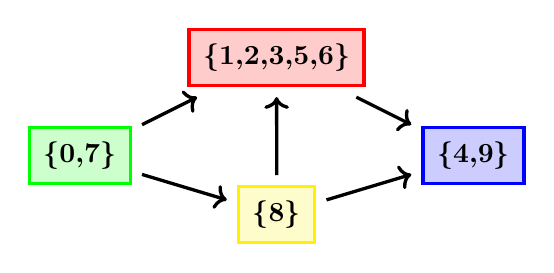
\begin{tikzpicture}
	[scale=2.5,very thick,every node/.style={draw,inner sep=0.18cm,outer sep=1.5mm}, every path/.style={->}]

	%\draw[help lines] (-1,-2) grid (7,2);
    \node[rectangle,green,fill=green!20] (0) at (0,0) {\color{black}\textbf{\{0,7\}}};
    \node[rectangle,red,fill=red!20] (1) at (1,0.5) {\color{black}\textbf{\{1,2,3,5,6\}}};
    \node[rectangle,blue,fill=blue!20] (4) at (2,0) {\color{black}\textbf{\{4,9\}}};
    \node[rectangle,yellow,fill=yellow!20] (8) at (1,-0.3) {\color{black}\textbf{\{8\}}};

    \path (0) edge (1);
    \path (0) edge (8);
    \path (1) edge (4);
    \path (8) edge (1);
    \path (8) edge (4);

\end{tikzpicture}

\end{document}
